\documentclass[11pt,a4paper]{article}
\usepackage[margin=2.2cm]{geometry}
\usepackage{lmodern}
\usepackage[T1]{fontenc}
\usepackage{amsmath,amssymb}
\usepackage{booktabs,array,float}
\usepackage[table]{xcolor}
\usepackage{graphicx}
\usepackage[font=small,labelfont=bf]{caption}
\usepackage{enumitem}
\usepackage{microtype}
\usepackage[colorlinks=true,linkcolor=blue!50!black,urlcolor=blue!50!black]{hyperref}

\definecolor{sel}{RGB}{222,236,252}
\newcommand{\why}{\textit{Why:} }
\newcommand{\decided}[1]{\textcolor{green!40!black}{\textbf{Decided:} #1}}
\newcommand{\RMS}{\operatorname{RMS}}
\newcommand{\avg}{\mathrm{avg}}
\setlist{itemsep=2pt,topsep=3pt}
\graphicspath{{main_figs/}{figs/}}

% two figures side by side
\newcommand{\figpair}[4]{%
\begin{figure}[H]\centering
\begin{minipage}[t]{0.48\textwidth}\centering\includegraphics[width=\linewidth]{#1}\caption{#2}\end{minipage}\hfill
\begin{minipage}[t]{0.48\textwidth}\centering\includegraphics[width=\linewidth]{#3}\caption{#4}\end{minipage}
\end{figure}}
\newcommand{\figone}[3][0.6]{%
\begin{figure}[H]\centering\includegraphics[width=#1\textwidth]{#2}\caption{#3}\end{figure}}

\title{Lithium Diffusion in a Spherical Particle:\\Effect of Flux Shape, Frequency and Diffusivity}
\author{Ishitva Yadav\\CL 443 \ --- \ Supervisor: Prof.\ Jason Picardo}
\date{October 30, 2026}

\begin{document}
\maketitle

%=====================================================================
\section{Problem}
Lithium diffusion inside a spherical particle is studied using a PDE model. The concentration inside the particle varies with radius and time, and lithium enters or leaves only through the surface. The outputs looked at are the surface concentration $C_s$, the average concentration $C_\avg$, and the concentration profile $C(r)$ inside the particle. Different flux inputs and different diffusivity values are applied to the same particle to see how they change the response. Six experiments are reported. Experiments 1 to 4 change one thing at a time (24 PDE simulations). Experiments 5 and 6 build two-equation models for $C_s$ and $C_\avg$, by the Galerkin method and by SINDy, and test them against further PDE simulations.

%=====================================================================
\section{Model}
The model is Fick's second law in spherical coordinates, written in dimensionless form. The scalings used are
\begin{equation}
  \tau = \frac{D_0 t}{R^2},\qquad r=\frac{\tilde r}{R},\qquad C=\frac{c}{c_0},\qquad f(C)=\frac{D(c)}{D_0},\qquad \delta = \frac{jR}{D_0c_0},
\end{equation}
so $\tau$ is scaled time, $r$ runs from 0 at the centre to 1 at the surface, $C$ is concentration as a fraction of full, $f(C)$ is the diffusivity relative to the reference value $D_0$, and $\delta$ is the scaled surface flux. The governing equation is
\begin{equation}\label{eq:pde}
  \frac{\partial C}{\partial\tau} = \frac{1}{r^2}\frac{\partial}{\partial r}\left[r^2 f(C)\frac{\partial C}{\partial r}\right],
\end{equation}
with boundary and initial conditions
\begin{align}
  f(C)\left.\frac{\partial C}{\partial r}\right|_{r=1} &= -\delta(\tau),\\
  \left.\frac{\partial C}{\partial r}\right|_{r=0} &= 0,\\
  C(r,0) &= 1.
\end{align}
The two reported quantities are
\begin{equation}
  C_s(\tau) = C(1,\tau),\qquad C_\avg(\tau) = 3\int_0^1 C(r,\tau)\,r^2\,dr.
\end{equation}
Integrating Equation~\eqref{eq:pde} over the particle and using the boundary conditions gives
\begin{equation}\label{eq:massbal}
  \frac{dC_\avg}{d\tau} = -3\,\delta(\tau),
\end{equation}
which ties the average concentration directly to the applied flux.

\subsection{Parameters}
The particle radius is $R=2\times10^{-6}$ m, the maximum concentration is $c_0=51554$ mol m$^{-3}$, and the reference diffusivity is $D_0=2\times10^{-14}$ m$^2$ s$^{-1}$. These give $R^2/D_0=200$ s, so one unit of $\tau$ is 200 seconds. The particle starts full and uniform, $C_0=1$, and each run of Experiments 1 to 4 covers $0\le\tau\le10$, that is 2000 seconds. The reference surface flux is $j_0=4.3\times10^{-6}$ mol m$^{-2}$ s$^{-1}$, which gives $\delta_0=j_0R/(D_0c_0)=0.008341$. A C-rate multiplier of 3 is used, so the flux amplitude in every deterministic profile is
\begin{equation}
  A = 3\,\delta_0 = 0.025022.
\end{equation}
The equations are solved in MATLAB using \texttt{pdepe} in spherical mode on a grid of 1000 radial points and 2000 time points, with relative and absolute tolerances of $10^{-9}$ and a maximum step of $10^{-2}$ in $\tau$. These settings are the same for all 24 runs of Experiments 1 to 4. Experiments 5 and 6 use their own run lengths and time steps, given there.

\subsection{Diffusivity}
Unless stated otherwise the diffusivity is the fitted NMC811 curve used in the solver:
\begin{equation}\label{eq:nmc}
  f(C) = p_4 + (p_1-p_4)\exp\left[-\exp\left(-p_2(C-p_3)\right)\right],
\end{equation}
with $p_1=0.1008$, $p_2=-8.2105$, $p_3=0.6986$ and $p_4=0.0009$. The NMC811 diffusivity is concentration dependent and is used as the default material model. It is low near $C=1$, about 0.0009, and rises to about 0.1 at low $C$. Experiment 3 replaces it with a constant $f$.

\subsection{Flux profiles}
Six deterministic flux shapes are used:
\begin{align}
  \texttt{const}:&\quad \delta(\tau)=A,\\
  \texttt{stepUp}:&\quad \delta(\tau)=A\left[1+\tfrac12\tanh 20(\tau-5)\right],\\
  \texttt{linear}:&\quad \delta(\tau)=A\,\frac{\tau}{10},\\
  \texttt{linearDown}:&\quad \delta(\tau)=A\left(1-\frac{\tau}{10}\right),\\
  \texttt{sin}:&\quad \delta(\tau)=A\sin(\omega\tau),\\
  \texttt{cos}:&\quad \delta(\tau)=A\cos(\omega\tau).
\end{align}
The frequency is $\omega=20$ everywhere except in Experiment 2, where it is swept. Since \texttt{sin} and \texttt{cos} are negative for half of each cycle, they push lithium back into the particle, so $C$ can rise above 1 in those runs. The model puts no upper bound on $C$.

%=====================================================================
\clearpage
\section{Experiment 1: flux shape}
\begin{itemize}
  \item The six flux profiles were applied to the same particle with the same diffusivity model.
  \item Only the shape of $\delta(\tau)$ was changed; $\omega=20$ for \texttt{sin} and \texttt{cos}.
\end{itemize}
\figpair{fig01}{The six applied flux profiles $\delta(\tau)$.}{fig02}{Surface concentration $C_s$ against $\tau$.}
\figpair{fig03}{Average concentration $C_\avg$ against $\tau$.}{fig04}{$C_s$ and $C_\avg$ against $\tau$.}
\figone{fig05}{$C_\avg-C_s$ against $\tau$.}
\begin{itemize}
  \item $C_s$ changes with the flux shape, while $C_\avg$ follows the total charge applied.
  \item \texttt{const} and \texttt{stepUp}: same charge 0.7507, same final $C_\avg=0.2493$, but $C_s$ minima of 0.1981 and 0.1704.
  \item \texttt{linear} and \texttt{linearDown}: same charge 0.3753, same final $C_\avg=0.6247$, but $C_s$ minima of 0.5158 and 0.5999.
  \item This follows from Equation~\eqref{eq:massbal}: $C_\avg$ depends only on the integral of $\delta$.
  \item Profiles that load the surface harder or earlier give a larger gap. \texttt{linearDown} peaks at $\tau=0$, where the diffusivity is lowest, and reaches a maximum gap of 0.2140 against 0.1736 for \texttt{const}.
\end{itemize}

\subsection{Inside the particle}
\begin{itemize}
  \item $r=0$ is the centre and $r=1$ is the surface.
  \item A flat curve means the particle is uniform; a drop near $r=1$ means the surface is emptied faster than diffusion refills it.
\end{itemize}
\figpair{fig06}{Concentration profile at $\tau=2$.}{fig07}{Concentration profile at $\tau=6$.}
\figone{fig08}{Concentration profile at $\tau=10$.}
\begin{itemize}
  \item The steady and ramped profiles change the concentration across the whole particle.
  \item \texttt{sin} and \texttt{cos} disturb only a thin layer near the surface and leave the interior close to its initial value.
\end{itemize}

%=====================================================================
\clearpage
\section{Experiment 2: frequency of the oscillating flux}
\begin{itemize}
  \item The flux was fixed at $\delta(\tau)=A\sin(\omega\tau)$ and only $\omega$ was changed, taking 2, 5, 10, 20, 40 and 80.
  \item The material model and all other solver settings were kept fixed.
  \item The period is $T_\tau=2\pi/\omega$, which gives 628.3, 251.3, 125.7, 62.8, 31.4 and 15.7 seconds.
  \item The time plots use the window $5\le\tau\le6$ (200 seconds), because at $\omega=80$ the full run holds more than 120 oscillations. Line thickness decreases as $\omega$ increases. The full solution is kept in the saved data.
\end{itemize}
\figpair{fig09}{Applied flux $\delta(\tau)$ for the six frequencies.}{fig10}{Surface concentration $C_s$ against $\tau$.}
\figpair{fig11}{Surface concentration $C_s$ against applied flux $\delta$.}{fig12}{Average concentration $C_\avg$ against $\tau$.}
\figpair{fig13}{Average concentration $C_\avg$ against applied flux $\delta$.}{fig14}{$C_\avg-C_s$ against $\tau$.}
\figone{fig15}{Concentration profiles at $\tau=2$, 6 and 10.}
\begin{itemize}
  \item Increasing $\omega$ reduces the visible oscillation in $C_s$: it spans 0.729 to 1.618 at $\omega=2$ and 0.889 to 1.092 at $\omega=80$, with the intermediate cases in order.
  \item $C_\avg$ changes very little. Its minimum rises from 0.925 to 0.998, because a faster oscillation reverses sign before much charge has accumulated.
  \item $C_s$ against $\delta$ is a loop, not a single line, so $C_s$ is not set by the instantaneous flux alone. The loops shrink as $\omega$ increases.
  \item The disturbed region moves closer to the surface: the profile is curved from about $r=0.55$ at $\omega=2$, and flat until about $r=0.97$ at $\omega=80$.
  \item The maximum gap $C_\avg-C_s$ falls from 0.215 to 0.110.
\end{itemize}

%=====================================================================
\clearpage
\section{Experiment 3: constant diffusivity}
\begin{itemize}
  \item Equation~\eqref{eq:nmc} was replaced by a constant, so $f(C)=f$ at every concentration, taking 0.01, 0.1, 1, 10 and 100.
  \item The flux was fixed at $\delta(\tau)=A\sin(20\tau)$ and all other settings were kept fixed.
  \item $D_0$ was not changed, so all five runs share the same time axis. The same window $5\le\tau\le6$ is used.
\end{itemize}
\figpair{fig16}{The five constant diffusivity levels (log vertical axis).}{fig17}{Surface concentration $C_s$ against $\tau$.}
\figpair{fig18}{Surface concentration $C_s$ against applied flux $\delta$.}{fig19}{Average concentration $C_\avg$ against $\tau$.}
\figpair{fig20}{Average concentration $C_\avg$ against applied flux $\delta$.}{fig21}{Concentration profiles at $\tau=2$, 6 and 10.}
\figone{fig22}{$C_\avg-C_s$ against $\tau$.}
\begin{itemize}
  \item At low diffusivity the profile is strongly non-uniform near the surface. As $f$ increases the gradient becomes smaller and the profile approaches a flat line.
  \item At $f=0.01$ the profile is flat through the interior and turns sharply in the last few percent of the radius, reaching 1.05 at the surface at $\tau=10$ while the centre sits near 0.996. At $f=100$ it is flat across the whole radius.
  \item The $C_s$ range narrows with $f$: 0.9228--1.0527, then 0.9740--1.0148, 0.9897--1.0028, 0.9924--1.0001 and 0.99249--1.00000.
  \item The maximum gap $C_\avg-C_s$ falls from 0.0710 to 0.0198, 0.00418, 0.000499 and 0.000051.
  \item The $C_\avg$ histories are essentially the same in all five runs, spanning 0.99249 to 1.00000 with a final value of 0.99808, because the applied flux is the same and Equation~\eqref{eq:massbal} contains no diffusivity.
\end{itemize}

%=====================================================================
\clearpage
\section{Experiment 4: randomly generated flux}
\begin{itemize}
  \item \texttt{trueRandom} generates a reproducible piecewise-constant flux from a fixed seed. It divides the run into 17 segments of random length and gives each segment a random amplitude.
  \item Changing the seed gives a different excitation while the generation method and all solver settings stay unchanged. This is useful for generating varied input--output data for later modelling.
  \item Five seeds were used: 30303, the original seed in the project and the reference case, then 101, 202, 303 and 404.
  \item Only the flux and the surface concentration are plotted.
  \item The amplitude convention differs from the deterministic profiles: an internal constant of 0.01 is used instead of $A=0.025022$, and the mean is subtracted from the amplitude sequence. The net charge removed is $-0.024$ to $+0.018$, against 0.751 for a steady discharge at $\delta=A$, so these are excitation signals rather than discharges and should not be compared directly with Experiment 1.
\end{itemize}

\subsection{Individual seeds}
\figpair{fig23}{Seed 30303 (reference). Applied flux $\delta(\tau)$.}{fig24}{Seed 30303. Surface concentration $C_s$.}
\figpair{fig25}{Seed 101. Applied flux $\delta(\tau)$.}{fig26}{Seed 101. Surface concentration $C_s$.}
\figpair{fig27}{Seed 202. Applied flux $\delta(\tau)$.}{fig28}{Seed 202. Surface concentration $C_s$.}
\figpair{fig29}{Seed 303. Applied flux $\delta(\tau)$.}{fig30}{Seed 303. Surface concentration $C_s$.}
\figpair{fig31}{Seed 404. Applied flux $\delta(\tau)$.}{fig32}{Seed 404. Surface concentration $C_s$.}

\subsection{All seeds together}
\figpair{fig33}{Applied flux $\delta(\tau)$ for all five seeds.}{fig34}{Surface concentration $C_s$ for all five seeds.}
\begin{itemize}
  \item The five fluxes differ from each other, with segment edges at different times and different sign patterns.
  \item The surface responses are similar in character: irregular excursions above and below $C_s=1$ with no steady drift.
  \item Across the five seeds $C_s$ spans 0.803 to 1.460 and $C_\avg$ spans 0.949 to 1.049.
  \item The minimum of $C_s$ varies only between 0.803 and 0.862, while the maximum varies more widely, between 1.158 and 1.460.
  \item Five seeds only show that the behaviour is similar in character, not anything about its distribution. The per-seed values are saved in \texttt{Results/tables/trueRandom\_summary.csv}.
\end{itemize}

%=====================================================================
\clearpage
\section{Experiment 5: two-equation model by the Galerkin method}
\begin{itemize}
  \item The aim is a model of two ordinary differential equations, one for $C_\avg$ and one for $C_s$, derived from the PDE by the Galerkin method, and then tested against the PDE.
  \item The diffusivity is constant, $f=1$, throughout this experiment and Experiment 6.
\end{itemize}

\subsection{Starting point: the Galerkin formulas}
\begin{itemize}
  \item The concentration is approximated by $N$ fixed radial shapes $P_k(r)$, each multiplied by a coefficient that depends only on time:
  \begin{equation}
    C(r,\tau)\approx\sum_{k=1}^{N}\alpha_k(\tau)\,P_k(r).
  \end{equation}
  \item The shapes are orthogonal with the spherical weight $r^2$, and the first shape is $P_1=1$:
  \begin{equation}\label{eq:orth}
    \int_0^1 r^2\,P_i(r)\,P_j(r)\,dr = 0\quad(i\neq j),\qquad P_1(r)=1.
  \end{equation}
  \item The Galerkin projection of the PDE onto these shapes gives the following two results, in dimensionless form. They are the starting point of this experiment.
  \begin{equation}\label{eq:galCs}
    \frac{dC_s}{d\tau} = -\delta(\tau)\sum_{i=1}^{N}\frac{P_i(1)^2}{\int_0^1 r^2P_i(r)^2\,dr}
    - \sum_{i=1}^{N}\frac{P_i(1)\int_0^1 r^2 P_i'(r)\, f\!\left(\sum_{k=1}^{N}\alpha_kP_k(r)\right)\left(\sum_{k=1}^{N}\alpha_kP_k'(r)\right)dr}{\int_0^1 r^2P_i(r)^2\,dr},
  \end{equation}
  \begin{equation}\label{eq:galCavg}
    \frac{dC_\avg}{d\tau} = \frac{d\alpha_1}{d\tau} = \frac{-\delta(\tau)}{\int_0^1 r^2\,dr} = -3\,\delta(\tau).
  \end{equation}
  \item $f(\cdot)$ is the diffusivity evaluated at the approximate concentration. With constant $f$, it is taken out of the integral in Equation~\eqref{eq:galCs}.
  \item Equation~\eqref{eq:galCavg} is the exact mass balance, Equation~\eqref{eq:massbal}.
  \item Equation~\eqref{eq:galCs} gives $dC_s/d\tau$ in terms of the coefficients $\alpha_k$. To obtain a model in $C_s$ and $C_\avg$, the shapes are chosen and the $\alpha_k$ are written in terms of $C_s$ and $C_\avg$.
\end{itemize}

\subsection{Choice of shapes, $N=2$}
\begin{itemize}
  \item $P_1=1$. The second shape is taken as $P_2=r^2+c$, the simplest shape that is even in $r$ (so $\partial C/\partial r=0$ at the centre) and can bend.
  \item The constant $c$ is fixed by the orthogonality condition, Equation~\eqref{eq:orth}, between $P_1$ and $P_2$:
  \begin{equation}
    \int_0^1 r^2\cdot1\cdot(r^2+c)\,dr = \frac15+\frac c3 = 0\quad\Rightarrow\quad c=-\frac35,\qquad P_1(r)=1,\qquad P_2(r)=r^2-\frac35.
  \end{equation}
  \item The approximation is $C=\alpha_1+\alpha_2\left(r^2-\frac35\right)$, a parabola in $r$.
\end{itemize}

\subsection{Linking $\alpha_1$, $\alpha_2$ to $C_\avg$ and $C_s$}
\textbf{Average concentration.} Using the definition $C_\avg=3\int_0^1C(r,\tau)\,r^2\,dr$ and the approximation:
\begin{equation}
  C_\avg = 3\left[\alpha_1\int_0^1r^2\,dr+\alpha_2\int_0^1r^2\left(r^2-\tfrac35\right)dr\right] = 3\left[\frac{\alpha_1}{3}+\alpha_2\cdot0\right]=\alpha_1.
\end{equation}
\begin{itemize}
  \item The second integral is zero by the orthogonality condition, since $\int_0^1r^2P_2\,dr=\int_0^1r^2P_1P_2\,dr=0$. So the first coefficient is exactly the average concentration, $\alpha_1=C_\avg$, which is why Equation~\eqref{eq:galCavg} is written as $dC_\avg/d\tau$.
\end{itemize}
\textbf{Surface concentration.} At $r=1$:
\begin{equation}
  C_s = \alpha_1P_1(1)+\alpha_2P_2(1) = \alpha_1+\frac25\,\alpha_2.
\end{equation}
\begin{itemize}
  \item With $\alpha_1=C_\avg$:
  \begin{equation}\label{eq:alphas}
    \alpha_1 = C_\avg,\qquad \alpha_2=\frac52\left(C_s-C_\avg\right).
  \end{equation}
\end{itemize}

\subsection{Applying the formula for $dC_s/d\tau$}
\begin{table}[H]\centering
\begin{tabular}{lccc}\toprule
 & $P_i(1)$ & $\int_0^1r^2P_i^2\,dr$ & $P_i'(r)$\\\midrule
$P_1=1$ & 1 & 1/3 & 0\\
$P_2=r^2-3/5$ & 2/5 & 4/175 & $2r$\\\bottomrule
\end{tabular}
\caption{Values needed in Equation~\eqref{eq:galCs}.}
\end{table}
\begin{itemize}
  \item $\int_0^1r^2P_2^2\,dr=\int_0^1\left(r^6-\frac65r^4+\frac9{25}r^2\right)dr=\frac17-\frac6{25}+\frac3{25}=\frac4{175}$.
  \item \textbf{First sum (flux term):}
  \[
    \frac{P_1(1)^2}{1/3}+\frac{P_2(1)^2}{4/175} = \frac1{1/3}+\frac{4/25}{4/175}=3+7=10.
  \]
  \item \textbf{Second sum (diffusion term).} Since $P_1'=0$, only $i=2$ contributes, and inside the bracket only $k=2$ contributes: $\sum_k\alpha_kP_k'(r)=2r\,\alpha_2$. With constant $f$:
  \[
    \frac{P_2(1)\,f\int_0^1r^2\,(2r)(2r\,\alpha_2)\,dr}{4/175} = \frac{\frac25\cdot\frac45\,f\,\alpha_2}{4/175} = 14\,f\,\alpha_2.
  \]
  \item So Equation~\eqref{eq:galCs} becomes
  \[
    \frac{dC_s}{d\tau} = -10\,\delta-14\,f\,\alpha_2.
  \]
  \item Replace $\alpha_2$ using Equation~\eqref{eq:alphas}: $14f\alpha_2=14f\cdot\frac52(C_s-C_\avg)=35f(C_s-C_\avg)$.
\end{itemize}

\subsection{The two-equation Galerkin model}
\begin{equation}\label{eq:galerkin}
  \boxed{\ \frac{dC_\avg}{d\tau}=-3\,\delta(\tau),\qquad \frac{dC_s}{d\tau}=-35f\left(C_s-C_\avg\right)-10\,\delta(\tau),\qquad C_s(0)=C_\avg(0)=1.\ }
\end{equation}
\begin{itemize}
  \item With $f=1$, written term by term: $dC_s/d\tau=-35\,C_s+35\,C_\avg-10\,\delta$. These three coefficients are compared with SINDy in Experiment 6.
  \item The initial values follow from $C(r,0)=1$: $\alpha_1=1$, $\alpha_2=0$.
  \item Assumptions: constant $f$; the profile is a combination of 1 and $r^2$ at every instant; the particle starts uniform.
  \item Slow-flux check: when $\delta$ changes slowly, $C_s$ and $C_\avg$ move together, so $dC_s/d\tau\approx-3\delta$, which gives $C_s-C_\avg=-\delta/(5f)$.
  \item With $N=2$ the equation for $C_s$ contains only $C_s$, $C_\avg$ and $\delta$. With $N\ge3$ it would also contain $\alpha_3,\dots$, which cannot be written with $C_s$ and $C_\avg$ alone.
\end{itemize}

\subsection{Test against the PDE}\label{sec:exp5test}
\begin{itemize}
  \item The flux is $\delta(\tau)=A\cos(\omega\tau)$ at $\omega=0.5$, 1, 2, 3, 5, 10, 20, 30, 50, 100 and 200.
  \item Each run lasts $\tau_{\max}=\max(10,\ 5\text{ periods})$ with time step $\min(0.005,\ \text{period}/100)$, on the same 1000-point radial grid.
  \item The Galerkin model, Equation~\eqref{eq:galerkin}, is solved on the same time points, starting from $C_s=C_\avg=1$.
\end{itemize}

\subsubsection{Error measure}
For a predicted signal $\hat y$ and a reference $y$, sampled at the $n$ points $t_1,\dots,t_n$ of a time \emph{window} $W$,
\begin{equation}\label{eq:rel}
  \mathrm{Rel}_W(\hat y,y) = \frac{\RMS_W(\hat y-y)}{\max_W y-\min_W y},\qquad
  \RMS_W(e)=\sqrt{\frac1n\sum_{k=1}^{n}e(t_k)^2},
\end{equation}
given in \% ($100\times$Rel). The denominator is the \emph{band} of the reference: its maximum minus its minimum in the window. The numerator and the denominator use the same window, stated with every result. Here $\hat y=C_{s,\rm model}$ and $y=C_{s,\rm PDE}$:
\[
  \mathrm{Rel}\ (\%) = 100\times\frac{\RMS\big(C_{s,\rm model}-C_{s,\rm PDE}\big)}{\max C_{s,\rm PDE}-\min C_{s,\rm PDE}}.
\]
\begin{table}[H]\centering\small
\begin{tabular}{rccr}\toprule
$\omega$ & band of $C_{s,\rm PDE}$ (last period) & RMS absolute error (last period) & Rel (\%)\\\midrule
0.5 & 0.3006 & $3.99\times10^{-7}$ & 0.0001\\
1 & 0.1507 & $1.60\times10^{-6}$ & 0.0011\\
2 & 0.0763 & $6.37\times10^{-6}$ & 0.0084\\
3 & 0.0518 & $1.42\times10^{-5}$ & 0.0275\\
5 & 0.0329 & $3.85\times10^{-5}$ & 0.1172\\
10 & 0.0196 & $1.38\times10^{-4}$ & 0.7031\\
20 & 0.0130 & $3.90\times10^{-4}$ & 2.9984\\
30 & 0.0104 & $5.95\times10^{-4}$ & 5.7293\\
50 & 0.0078 & $7.95\times10^{-4}$ & 10.1721\\
100 & 0.0054 & $8.69\times10^{-4}$ & 16.1875\\
200 & 0.0037 & $7.79\times10^{-4}$ & 20.9499\\\bottomrule
\end{tabular}
\caption{Band of $C_{s,\rm PDE}$, absolute and relative error of the Galerkin model, last period.}
\end{table}

\subsubsection{Windows}
\begin{itemize}
  \item \textbf{Whole run:} from $\tau=0$, where the flux is switched on at full size on a uniform particle, to the end of the run.
  \item \textbf{Last period:} the last period of the run.
\end{itemize}

\subsubsection{Periodicity check}
With constant $f$ and a sine or cosine flux, consecutive periods of the PDE solution were compared, and the Galerkin error was computed over the last one and the last two periods:
\begin{table}[H]\centering\small
\begin{tabular}{rccc}\toprule
$\omega$ & $\max|C_s(\tau)-C_s(\tau-P)|$ over the last period & Rel \%, last 2 periods & Rel \%, last period\\\midrule
0.5 & $1.2\times10^{-7}$ & 0.0001 & 0.0001\\
3 & $4.3\times10^{-9}$ & 0.0275 & 0.0275\\
30 & $7.5\times10^{-8}$ & 5.717 & 5.729\\
200 & $8.9\times10^{-10}$ & 20.996 & 20.950\\\bottomrule
\end{tabular}
\caption{Periodicity of the PDE solution, and the Galerkin error over one and two periods.}
\end{table}
The last period is used from here on.

\subsubsection{Result}
\begin{table}[H]\centering\small
\begin{tabular}{r|cc|cc|cc}\toprule
 & \multicolumn{2}{c|}{$C_s$ range} & \multicolumn{2}{c|}{$\max|C_s-C_{s,\rm PDE}|$} & \multicolumn{2}{c}{Rel (\%)}\\
$\omega$ & PDE & Galerkin & whole run & last period & whole run & last period\\\midrule
0.5 & 0.84971--1.15029 & 0.84971--1.15029 & $9.50\times10^{-4}$ & $5.75\times10^{-7}$ & 0.005 & 0.0001\\
1 & 0.92463--1.07537 & 0.92463--1.07537 & $9.50\times10^{-4}$ & $2.29\times10^{-6}$ & 0.015 & 0.0011\\
2 & 0.96186--1.03814 & 0.96185--1.03815 & $9.50\times10^{-4}$ & $9.02\times10^{-6}$ & 0.043 & 0.0084\\
3 & 0.97408--1.02592 & 0.97407--1.02593 & $9.50\times10^{-4}$ & $2.01\times10^{-5}$ & 0.081 & 0.0275\\
5 & 0.98357--1.01643 & 0.98354--1.01646 & $9.50\times10^{-4}$ & $5.45\times10^{-5}$ & 0.172 & 0.1172\\
10 & 0.99022--1.00978 & 0.99003--1.00997 & $9.49\times10^{-4}$ & $1.95\times10^{-4}$ & 0.735 & 0.7031\\
20 & 0.99349--1.00652 & 0.99299--1.00701 & $9.40\times10^{-4}$ & $5.51\times10^{-4}$ & 2.998 & 2.9984\\
30 & 0.99481--1.00524 & 0.99425--1.00577 & $9.35\times10^{-4}$ & $8.37\times10^{-4}$ & 5.672 & 5.7293\\
50 & 0.99609--1.00398 & 0.99581--1.00427 & $1.13\times10^{-3}$ & $1.13\times10^{-3}$ & 10.109 & 10.1721\\
100 & 0.99732--1.00275 & 0.99763--1.00249 & $1.26\times10^{-3}$ & $1.23\times10^{-3}$ & 16.046 & 16.1875\\
200 & 0.99814--1.00191 & 0.99877--1.00130 & $1.13\times10^{-3}$ & $1.11\times10^{-3}$ & 20.752 & 20.9499\\\bottomrule
\end{tabular}
\caption{Galerkin model against the PDE, cosine flux, $f=1$.}
\label{tab:exp5}
\end{table}
\figpair{fig35}{$C_s$, PDE and Galerkin model, $\omega=3$.}{fig36}{$C_s$, PDE and Galerkin model, $\omega=30$.}

%=====================================================================
\clearpage
\section{Experiment 6: SINDy}
\begin{itemize}
  \item SINDy (sparse identification of nonlinear dynamics, Brunton, Proctor and Kutz, 2016) finds an equation directly from data. The time derivative of a quantity is written as a combination of candidate terms (the library), and only the terms that are needed are kept.
  \item The aim is to find the equation for $dC_s/d\tau$ from PDE data and compare its coefficients with the Galerkin model of Experiment 5.
  \item The SINDy code and the method of choosing $\lambda$ are first applied to the Lorenz system, whose equations are known.
\end{itemize}

\subsection{Method}
\begin{itemize}
  \item Data are collected at many times and stacked: $\dot X=\Theta(X)\,\Xi$, where each column of $\Theta$ is one candidate term evaluated on the data, and $\Xi$ holds the unknown coefficients.
  \item $\Xi$ is found by sequentially thresholded least squares (STLSQ): fit by least squares, set every coefficient smaller than a threshold $\lambda$ to zero, fit again using only the remaining terms, and repeat (10 times). The threshold is applied to the coefficients directly.
\end{itemize}

\subsubsection{Training, validation and test data}
\begin{itemize}
  \item \textbf{Training data}: the data SINDy is fitted on.
  \item \textbf{Validation data}: runs not used in the fit, used to score every model in the $\lambda$ sweep and to choose $\lambda$.
  \item \textbf{Test data}: a third set, used once, after $\lambda$ has been chosen.
\end{itemize}

\subsubsection{Model errors}
All errors use Equation~\eqref{eq:rel}. When there are several variables (for Lorenz $x$, $y$, $z$), Rel is computed for each variable separately, with its own band, and the results are averaged.
\begin{itemize}
  \item $E_{train}$: Rel of $\Theta(X)\Xi$ against the derivative it was fitted to, on the training data.
  \item $E_{dv}$ (derivative on validation data): Rel of $\Theta(X)\Xi$ against the derivative of the validation data, with $\Theta$ evaluated at the true states of the validation data.
  \item $E_{sim}$ (simulation on validation data): the SINDy equations are solved from the starting point of the validation data, and the solution is compared with the true states.
\end{itemize}
They are written out in full for Lorenz in Section~\ref{sec:lorenz-err} and for the PDE in Section~\ref{sec:pde-err}.

\subsubsection{The $\lambda$ grid}\label{sec:grid}
$\lambda$ is swept on a log scale with four values per decade, $\lambda_k=10^{k/4}$, so each step multiplies or divides $\lambda$ by $10^{0.25}\approx1.78$:
\[
  \dots,\ 0.178,\ 0.316,\ 0.562,\ 1.0,\ 1.78,\ 3.16,\ 5.62,\ 10,\ \dots
\]

\subsubsection{Rule for choosing $\lambda$}\label{sec:rule}
\begin{enumerate}
  \item \textbf{Sweep.} Run STLSQ for every $\lambda$ on the grid.
  \item \textbf{Merge.} $\lambda$ values that give the same model are merged into one model with a $\lambda$ range.
  \item \textbf{Score.} Compute each model's error on the validation data ($E_{dv}$ for Lorenz, $E_{sim}$ for the PDE).
  \item \textbf{Discard unstable models.} Remove models whose solution grows without bound when they are solved. The empty model (all coefficients zero) is kept.
  \item \textbf{Order.} Arrange the remaining models from largest to smallest $\lambda$.
  \item \textbf{Find the knee.} Between each pair of neighbours compute the drop in error, $\log_{10}E_{\rm before}-\log_{10}E_{\rm after}$, and find the largest drop.
  \item \textbf{Select.} Take the model just after the largest drop.
  \item \textbf{Choose $\lambda$.} Use the largest $\lambda$ of that model's range.
  \item \textbf{Test.} Score the selected model once on the test data.
\end{enumerate}
This rule is called R4 below. Three other rules are compared with it for Lorenz in Section~\ref{sec:rules}.

%---------------------------------------------------------------------
\subsection{Check on the Lorenz system}

\subsubsection{System, data and derivatives}
\begin{equation}
  \dot x=\sigma(y-x),\qquad \dot y = x(\rho-z)-y,\qquad \dot z=xy-\beta z,\qquad
  \sigma=10,\ \rho=28,\ \beta=8/3,
\end{equation}
starting from $x(0)=-8$, $y(0)=7$, $z(0)=27$. With these values the true equations are $\dot x=-10x+10y$, $\dot y=28x-y-xz$, $\dot z=-2.6667z+xy$: seven terms in total.
\begin{itemize}
  \item Training data every $\Delta t=0.001$ up to $t=100$ ($10^5$ points). Library: all polynomials in $x,y,z$ up to fifth order (56 terms, from 1 to $z^5$). 10 threshold-and-refit passes.
\end{itemize}
The derivatives $\dot X$ are obtained in three ways:
\begin{align*}
  \text{A (exact):}\quad & \dot X \text{ from the equations},\\
  \text{C2 (2nd-order central):}\quad & \dot X_i \approx \frac{X_{i+1}-X_{i-1}}{2\Delta t}, \qquad \text{error} \propto \Delta t^2,\\
  \text{C4 (4th-order central):}\quad & \dot X_i \approx \frac{-X_{i+2}+8X_{i+1}-8X_{i-1}+X_{i-2}}{12\,\Delta t}, \qquad \text{error}\propto\Delta t^4 .
\end{align*}
For C2 and C4 the one or two points at each end, where the central formula cannot be used, are left out.

\begin{table}[H]\centering\small
\begin{tabular}{llrrrr}\toprule Equation & Term & True & A (exact) & C2 (2nd order) & C4 (4th order)\\\midrule
$\dot x$ & $x$ & -10.0000 & -10.000000 & -9.999780 & -10.000000\\
$\dot x$ & $y$ & 10.0000 & 10.000000 & 9.999779 & 10.000000\\
$\dot y$ & $x$ & 28.0000 & 28.000000 & 27.997984 & 28.000000\\
$\dot y$ & $y$ & -1.0000 & -1.000000 & -0.999606 & -1.000000\\
$\dot y$ & $xz$ & -1.0000 & -1.000000 & -0.999944 & -1.000000\\
$\dot z$ & $z$ & -2.6667 & -2.666667 & -2.666589 & -2.666667\\
$\dot z$ & $xy$ & 1.0000 & 1.000000 & 0.999971 & 1.000000\\
\midrule max $|\xi_{\rm SINDy}-\xi_{\rm true}|$ & & & $5.2\!\times\!10^{-14}$ & $2.0\!\times\!10^{-3}$ & $2.3\!\times\!10^{-7}$\\
\bottomrule\end{tabular}
\caption{Lorenz coefficients of the model selected by R4 (Section~\ref{sec:lorenz-apply}). All other 161 coefficients are zero. Last row: maximum coefficient error (Section~\ref{sec:lorenz-err}).}
\label{tab:lorenz-coefs}
\end{table}

\subsubsection{Training, validation and test runs}
\begin{itemize}
  \item \textbf{Training:} the run above, from $(-8,7,27)$, $0\le t\le100$.
  \item \textbf{Validation:} three runs from $(5,-5,20)$, $(-3,4,30)$ and $(8,8,15)$, $0\le t\le 20$, $\Delta t=0.001$.
  \item \textbf{Test:} three runs from $(1,-1,25)$, $(-6,6,18)$ and $(10,3,32)$, $0\le t\le 20$, $\Delta t=0.001$.
\end{itemize}

\subsubsection{Error measures}\label{sec:lorenz-err}
$\dot x_{\rm ref}$ is the derivative of the data, taken by the same method as in training (A, C2 or C4), and $\dot x_{\rm SINDy}=\Theta(x,y,z)\,\xi_x$ is the SINDy equation for $\dot x$, evaluated at the true $x,y,z$ of the data; likewise for $y$ and $z$. The errors are given as fractions.

\textbf{Training error}, on the training run:
\[
  E_{train} = \frac13\left[
  \frac{\RMS(\dot x_{\rm SINDy}-\dot x_{\rm ref})}{\max\dot x_{\rm ref}-\min\dot x_{\rm ref}} +
  \frac{\RMS(\dot y_{\rm SINDy}-\dot y_{\rm ref})}{\max\dot y_{\rm ref}-\min\dot y_{\rm ref}} +
  \frac{\RMS(\dot z_{\rm SINDy}-\dot z_{\rm ref})}{\max\dot z_{\rm ref}-\min\dot z_{\rm ref}}\right].
\]

\textbf{Derivative error on validation data}: the same formula on each validation run $j=1,2,3$ (window: the whole run, $0\le t\le20$), averaged over the three runs:
\[
  E_{dv} = \frac13\sum_{j=1}^{3}\ \frac13\sum_{v\in\{x,y,z\}}
  \frac{\RMS\big(\dot v_{\rm SINDy}-\dot v_{\rm ref}\big)_j}{\big(\max \dot v_{\rm ref}-\min\dot v_{\rm ref}\big)_j}.
\]

\textbf{Simulation error on validation data}: the SINDy equations are solved from the starting point of validation run $j$, giving $x_{\rm SINDy}(t), y_{\rm SINDy}(t), z_{\rm SINDy}(t)$, which are compared with the true $x(t),y(t),z(t)$ over $0\le t\le T$, $T=0.5$, 1 and 2:
\[
  E_{sim}(T) = \frac13\sum_{j=1}^{3}\ \frac13\sum_{v\in\{x,y,z\}}
  \frac{\RMS_{[0,T]}\big(v_{\rm SINDy}-v\big)_j}{\big(\max_{[0,T]} v-\min_{[0,T]} v\big)_j}.
\]
A model whose solution grows without bound gets $E_{sim}=\infty$.

\textbf{Maximum coefficient error}: the largest of the $56\times3=168$ differences between the SINDy coefficients and the true ones,
\[
  \text{max coef.\ err.} = \max_{i,k} \big|\Xi_{ik,\rm SINDy}-\Xi_{ik,\rm true}\big| ,
\]
where the true $\Xi$ has the 7 Lorenz coefficients and 161 zeros.

$\lambda$ is chosen with $E_{dv}$; $E_{sim}$ is reported alongside.

\subsubsection{Sweeping the threshold}
$\lambda$ is swept from $10^{-12}$ to $10^{1.5}\approx 32$. Rows giving the same model are merged. ``Wrong'': a term not in the true equations. ``Missing'': a true term that was removed. Shaded: the model selected by R4 (Section~\ref{sec:lorenz-apply}).

\begin{table}[H]\centering\scriptsize\setlength{\tabcolsep}{4pt}
\resizebox{\textwidth}{!}{\begin{tabular}{lrrrrrrrrr}\toprule
$\lambda$ range & terms & wrong & missing & max coef.\ err. & $E_{train}$ & $E_{dv}$ & $E_{sim}(0.5)$ & $E_{sim}(1)$ & $E_{sim}(2)$\\\midrule
$1.0\!\times\!10^{1}$ -- $3.2\!\times\!10^{1}$ & 0 & 0 & 7 & $2.8\!\times\!10^{1}$ & $1.6\!\times\!10^{-1}$ & $1.6\!\times\!10^{-1}$ & $4.8\!\times\!10^{-1}$ & $3.9\!\times\!10^{-1}$ & $3.5\!\times\!10^{-1}$\\
$3.2\!\times\!10^{0}$ -- $5.6\!\times\!10^{0}$ & 2 & 0 & 5 & $2.8\!\times\!10^{1}$ & $1.0\!\times\!10^{-1}$ & $1.0\!\times\!10^{-1}$ & $4.1\!\times\!10^{-1}$ & $3.3\!\times\!10^{-1}$ & $3.2\!\times\!10^{-1}$\\
$1.8\!\times\!10^{0}$ & 3 & 0 & 4 & $3.1\!\times\!10^{1}$ & $1.0\!\times\!10^{-1}$ & $9.8\!\times\!10^{-2}$ & $4.5\!\times\!10^{-1}$ & $3.8\!\times\!10^{-1}$ & $3.1\!\times\!10^{-1}$\\
$1.0\!\times\!10^{0}$ & 6 & 0 & 1 & $4.1\!\times\!10^{1}$ & $2.7\!\times\!10^{-2}$ & $2.8\!\times\!10^{-2}$ & $6.3\!\times\!10^{-1}$ & $6.1\!\times\!10^{-1}$ & $5.0\!\times\!10^{-1}$\\
\rowcolor{sel}$1.0\!\times\!10^{-12}$ -- $5.6\!\times\!10^{-1}$ & 7 & 0 & 0 & $5.2\!\times\!10^{-14}$ & $2.2\!\times\!10^{-16}$ & $2.2\!\times\!10^{-16}$ & $4.8\!\times\!10^{-11}$ & $5.8\!\times\!10^{-11}$ & $2.0\!\times\!10^{-10}$\\
\bottomrule\end{tabular}}
\caption{Case A, exact derivative. Errors as fractions.}
\end{table}
\begin{table}[H]\centering\scriptsize\setlength{\tabcolsep}{4pt}
\resizebox{\textwidth}{!}{\begin{tabular}{lrrrrrrrrr}\toprule
$\lambda$ range & terms & wrong & missing & max coef.\ err. & $E_{train}$ & $E_{dv}$ & $E_{sim}(0.5)$ & $E_{sim}(1)$ & $E_{sim}(2)$\\\midrule
$1.0\!\times\!10^{1}$ -- $3.2\!\times\!10^{1}$ & 0 & 0 & 7 & $2.8\!\times\!10^{1}$ & $1.6\!\times\!10^{-1}$ & $1.6\!\times\!10^{-1}$ & $4.8\!\times\!10^{-1}$ & $3.9\!\times\!10^{-1}$ & $3.5\!\times\!10^{-1}$\\
$3.2\!\times\!10^{0}$ -- $5.6\!\times\!10^{0}$ & 2 & 0 & 5 & $2.8\!\times\!10^{1}$ & $1.0\!\times\!10^{-1}$ & $1.0\!\times\!10^{-1}$ & $4.1\!\times\!10^{-1}$ & $3.3\!\times\!10^{-1}$ & $3.2\!\times\!10^{-1}$\\
$1.0\!\times\!10^{0}$ -- $1.8\!\times\!10^{0}$ & 3 & 0 & 4 & $3.1\!\times\!10^{1}$ & $1.0\!\times\!10^{-1}$ & $9.8\!\times\!10^{-2}$ & $4.5\!\times\!10^{-1}$ & $3.8\!\times\!10^{-1}$ & $3.1\!\times\!10^{-1}$\\
\rowcolor{sel}$5.6\!\times\!10^{-5}$ -- $5.6\!\times\!10^{-1}$ & 7 & 0 & 0 & $2.0\!\times\!10^{-3}$ & $4.8\!\times\!10^{-6}$ & $4.9\!\times\!10^{-6}$ & $2.3\!\times\!10^{-5}$ & $5.4\!\times\!10^{-5}$ & $1.0\!\times\!10^{-4}$\\
$3.2\!\times\!10^{-5}$ & 8 & 1 & 0 & $2.0\!\times\!10^{-3}$ & $4.6\!\times\!10^{-6}$ & $4.7\!\times\!10^{-6}$ & $2.1\!\times\!10^{-5}$ & $6.1\!\times\!10^{-5}$ & $1.4\!\times\!10^{-4}$\\
$1.8\!\times\!10^{-5}$ & 9 & 2 & 0 & $2.0\!\times\!10^{-3}$ & $4.4\!\times\!10^{-6}$ & $4.5\!\times\!10^{-6}$ & $2.1\!\times\!10^{-5}$ & $5.4\!\times\!10^{-5}$ & $1.3\!\times\!10^{-4}$\\
$1.0\!\times\!10^{-5}$ & 12 & 5 & 0 & $2.8\!\times\!10^{-3}$ & $3.8\!\times\!10^{-6}$ & $3.9\!\times\!10^{-6}$ & $4.6\!\times\!10^{-5}$ & $7.1\!\times\!10^{-5}$ & $1.7\!\times\!10^{-4}$\\
$5.6\!\times\!10^{-6}$ & 14 & 7 & 0 & $2.8\!\times\!10^{-3}$ & $2.3\!\times\!10^{-6}$ & $2.5\!\times\!10^{-6}$ & $4.7\!\times\!10^{-5}$ & $5.7\!\times\!10^{-5}$ & $1.3\!\times\!10^{-4}$\\
$1.8\!\times\!10^{-6}$ -- $3.2\!\times\!10^{-6}$ & 17 & 10 & 0 & $1.2\!\times\!10^{-3}$ & $1.2\!\times\!10^{-6}$ & $1.4\!\times\!10^{-6}$ & $1.8\!\times\!10^{-5}$ & $4.5\!\times\!10^{-5}$ & $8.6\!\times\!10^{-5}$\\
$1.8\!\times\!10^{-7}$ -- $1.0\!\times\!10^{-6}$ & 19 & 12 & 0 & $3.7\!\times\!10^{-3}$ & $3.3\!\times\!10^{-7}$ & $3.6\!\times\!10^{-7}$ & $1.8\!\times\!10^{-5}$ & $2.7\!\times\!10^{-5}$ & $3.1\!\times\!10^{-5}$\\
$1.8\!\times\!10^{-9}$ -- $1.0\!\times\!10^{-7}$ & 21 & 14 & 0 & $1.8\!\times\!10^{-3}$ & $1.3\!\times\!10^{-10}$ & $1.4\!\times\!10^{-10}$ & $2.3\!\times\!10^{-5}$ & $3.1\!\times\!10^{-5}$ & $3.5\!\times\!10^{-5}$\\
$1.0\!\times\!10^{-9}$ & 22 & 15 & 0 & $1.8\!\times\!10^{-3}$ & $1.3\!\times\!10^{-10}$ & $1.3\!\times\!10^{-10}$ & $2.3\!\times\!10^{-5}$ & $3.1\!\times\!10^{-5}$ & $3.5\!\times\!10^{-5}$\\
$5.6\!\times\!10^{-10}$ & 23 & 16 & 0 & $1.8\!\times\!10^{-3}$ & $1.3\!\times\!10^{-10}$ & $1.3\!\times\!10^{-10}$ & $2.3\!\times\!10^{-5}$ & $3.1\!\times\!10^{-5}$ & $3.5\!\times\!10^{-5}$\\
$3.2\!\times\!10^{-10}$ & 24 & 17 & 0 & $1.8\!\times\!10^{-3}$ & $1.3\!\times\!10^{-10}$ & $1.3\!\times\!10^{-10}$ & $2.3\!\times\!10^{-5}$ & $3.1\!\times\!10^{-5}$ & $3.5\!\times\!10^{-5}$\\
$1.0\!\times\!10^{-10}$ & 32 & 25 & 0 & $1.8\!\times\!10^{-3}$ & $1.1\!\times\!10^{-10}$ & $1.2\!\times\!10^{-10}$ & $2.3\!\times\!10^{-5}$ & $3.1\!\times\!10^{-5}$ & $3.5\!\times\!10^{-5}$\\
$5.6\!\times\!10^{-11}$ & 42 & 35 & 0 & $1.8\!\times\!10^{-3}$ & $1.0\!\times\!10^{-10}$ & $1.1\!\times\!10^{-10}$ & $2.3\!\times\!10^{-5}$ & $3.1\!\times\!10^{-5}$ & $3.5\!\times\!10^{-5}$\\
$3.2\!\times\!10^{-11}$ & 38 & 31 & 0 & $1.8\!\times\!10^{-3}$ & $8.7\!\times\!10^{-11}$ & $9.8\!\times\!10^{-11}$ & $2.3\!\times\!10^{-5}$ & $3.1\!\times\!10^{-5}$ & $3.5\!\times\!10^{-5}$\\
$1.8\!\times\!10^{-11}$ & 46 & 39 & 0 & $1.8\!\times\!10^{-3}$ & $3.2\!\times\!10^{-11}$ & $3.9\!\times\!10^{-11}$ & $2.3\!\times\!10^{-5}$ & $3.1\!\times\!10^{-5}$ & $3.5\!\times\!10^{-5}$\\
$1.0\!\times\!10^{-11}$ & 53 & 46 & 0 & $1.8\!\times\!10^{-3}$ & $3.0\!\times\!10^{-11}$ & $3.7\!\times\!10^{-11}$ & $2.3\!\times\!10^{-5}$ & $3.1\!\times\!10^{-5}$ & $3.5\!\times\!10^{-5}$\\
$5.6\!\times\!10^{-12}$ & 60 & 53 & 0 & $1.8\!\times\!10^{-3}$ & $2.1\!\times\!10^{-11}$ & $2.6\!\times\!10^{-11}$ & $2.3\!\times\!10^{-5}$ & $3.1\!\times\!10^{-5}$ & $3.5\!\times\!10^{-5}$\\
$3.2\!\times\!10^{-12}$ & 62 & 55 & 0 & $1.8\!\times\!10^{-3}$ & $1.6\!\times\!10^{-11}$ & $2.0\!\times\!10^{-11}$ & $2.3\!\times\!10^{-5}$ & $3.1\!\times\!10^{-5}$ & $3.5\!\times\!10^{-5}$\\
$1.8\!\times\!10^{-12}$ & 58 & 51 & 0 & $1.8\!\times\!10^{-3}$ & $6.5\!\times\!10^{-12}$ & $9.4\!\times\!10^{-12}$ & $2.3\!\times\!10^{-5}$ & $3.1\!\times\!10^{-5}$ & $3.5\!\times\!10^{-5}$\\
$1.0\!\times\!10^{-12}$ & 64 & 57 & 0 & $1.8\!\times\!10^{-3}$ & $6.4\!\times\!10^{-12}$ & $9.5\!\times\!10^{-12}$ & $2.3\!\times\!10^{-5}$ & $3.1\!\times\!10^{-5}$ & $3.5\!\times\!10^{-5}$\\
\bottomrule\end{tabular}}
\caption{Case C2, 2nd-order finite differences.}
\end{table}
\begin{table}[H]\centering\scriptsize\setlength{\tabcolsep}{4pt}
\resizebox{\textwidth}{!}{\begin{tabular}{lrrrrrrrrr}\toprule
$\lambda$ range & terms & wrong & missing & max coef.\ err. & $E_{train}$ & $E_{dv}$ & $E_{sim}(0.5)$ & $E_{sim}(1)$ & $E_{sim}(2)$\\\midrule
$1.0\!\times\!10^{1}$ -- $3.2\!\times\!10^{1}$ & 0 & 0 & 7 & $2.8\!\times\!10^{1}$ & $1.6\!\times\!10^{-1}$ & $1.6\!\times\!10^{-1}$ & $4.8\!\times\!10^{-1}$ & $3.9\!\times\!10^{-1}$ & $3.5\!\times\!10^{-1}$\\
$3.2\!\times\!10^{0}$ -- $5.6\!\times\!10^{0}$ & 2 & 0 & 5 & $2.8\!\times\!10^{1}$ & $1.0\!\times\!10^{-1}$ & $1.0\!\times\!10^{-1}$ & $4.1\!\times\!10^{-1}$ & $3.3\!\times\!10^{-1}$ & $3.2\!\times\!10^{-1}$\\
$1.0\!\times\!10^{0}$ -- $1.8\!\times\!10^{0}$ & 3 & 0 & 4 & $3.1\!\times\!10^{1}$ & $1.0\!\times\!10^{-1}$ & $9.8\!\times\!10^{-2}$ & $4.5\!\times\!10^{-1}$ & $3.8\!\times\!10^{-1}$ & $3.1\!\times\!10^{-1}$\\
\rowcolor{sel}$1.8\!\times\!10^{-8}$ -- $5.6\!\times\!10^{-1}$ & 7 & 0 & 0 & $2.3\!\times\!10^{-7}$ & $1.1\!\times\!10^{-9}$ & $1.1\!\times\!10^{-9}$ & $2.7\!\times\!10^{-9}$ & $5.7\!\times\!10^{-9}$ & $1.2\!\times\!10^{-8}$\\
$1.0\!\times\!10^{-8}$ & 9 & 2 & 0 & $8.5\!\times\!10^{-7}$ & $1.1\!\times\!10^{-9}$ & $1.1\!\times\!10^{-9}$ & $2.5\!\times\!10^{-9}$ & $5.6\!\times\!10^{-9}$ & $1.7\!\times\!10^{-8}$\\
$5.6\!\times\!10^{-9}$ & 10 & 3 & 0 & $8.5\!\times\!10^{-7}$ & $1.1\!\times\!10^{-9}$ & $1.1\!\times\!10^{-9}$ & $2.5\!\times\!10^{-9}$ & $5.5\!\times\!10^{-9}$ & $1.7\!\times\!10^{-8}$\\
$3.2\!\times\!10^{-9}$ & 13 & 6 & 0 & $8.5\!\times\!10^{-7}$ & $9.7\!\times\!10^{-10}$ & $1.0\!\times\!10^{-9}$ & $5.1\!\times\!10^{-9}$ & $6.4\!\times\!10^{-9}$ & $1.8\!\times\!10^{-8}$\\
$1.8\!\times\!10^{-9}$ & 18 & 11 & 0 & $8.8\!\times\!10^{-7}$ & $5.5\!\times\!10^{-10}$ & $5.9\!\times\!10^{-10}$ & $4.9\!\times\!10^{-9}$ & $7.4\!\times\!10^{-9}$ & $1.2\!\times\!10^{-8}$\\
$1.0\!\times\!10^{-9}$ & 19 & 12 & 0 & $1.4\!\times\!10^{-6}$ & $5.5\!\times\!10^{-10}$ & $5.9\!\times\!10^{-10}$ & $4.8\!\times\!10^{-9}$ & $6.9\!\times\!10^{-9}$ & $1.0\!\times\!10^{-8}$\\
$5.6\!\times\!10^{-10}$ & 22 & 15 & 0 & $1.4\!\times\!10^{-6}$ & $6.0\!\times\!10^{-10}$ & $6.4\!\times\!10^{-10}$ & $3.7\!\times\!10^{-9}$ & $6.0\!\times\!10^{-9}$ & $1.4\!\times\!10^{-8}$\\
$3.2\!\times\!10^{-10}$ & 32 & 25 & 0 & $9.0\!\times\!10^{-7}$ & $4.7\!\times\!10^{-10}$ & $4.9\!\times\!10^{-10}$ & $2.9\!\times\!10^{-9}$ & $4.2\!\times\!10^{-9}$ & $1.5\!\times\!10^{-8}$\\
$1.8\!\times\!10^{-10}$ & 38 & 31 & 0 & $5.6\!\times\!10^{-7}$ & $3.6\!\times\!10^{-10}$ & $3.8\!\times\!10^{-10}$ & $8.1\!\times\!10^{-9}$ & $1.4\!\times\!10^{-8}$ & $1.9\!\times\!10^{-8}$\\
$1.0\!\times\!10^{-10}$ & 46 & 39 & 0 & $9.8\!\times\!10^{-8}$ & $2.3\!\times\!10^{-10}$ & $2.5\!\times\!10^{-10}$ & $4.2\!\times\!10^{-9}$ & $5.5\!\times\!10^{-9}$ & $9.2\!\times\!10^{-9}$\\
$5.6\!\times\!10^{-11}$ & 51 & 44 & 0 & $7.9\!\times\!10^{-7}$ & $1.3\!\times\!10^{-10}$ & $1.6\!\times\!10^{-10}$ & $2.2\!\times\!10^{-9}$ & $3.7\!\times\!10^{-9}$ & $7.3\!\times\!10^{-9}$\\
$3.2\!\times\!10^{-11}$ & 56 & 49 & 0 & $7.4\!\times\!10^{-7}$ & $1.2\!\times\!10^{-10}$ & $1.5\!\times\!10^{-10}$ & $2.1\!\times\!10^{-9}$ & $2.6\!\times\!10^{-9}$ & $4.0\!\times\!10^{-9}$\\
$1.8\!\times\!10^{-11}$ & 60 & 53 & 0 & $7.7\!\times\!10^{-7}$ & $8.4\!\times\!10^{-11}$ & $1.0\!\times\!10^{-10}$ & $3.1\!\times\!10^{-9}$ & $3.3\!\times\!10^{-9}$ & $5.5\!\times\!10^{-9}$\\
$1.0\!\times\!10^{-11}$ & 62 & 55 & 0 & $2.1\!\times\!10^{-6}$ & $3.9\!\times\!10^{-11}$ & $5.4\!\times\!10^{-11}$ & $1.8\!\times\!10^{-9}$ & $2.7\!\times\!10^{-9}$ & $4.7\!\times\!10^{-9}$\\
$5.6\!\times\!10^{-12}$ & 64 & 57 & 0 & $2.9\!\times\!10^{-6}$ & $2.4\!\times\!10^{-11}$ & $3.6\!\times\!10^{-11}$ & $1.4\!\times\!10^{-9}$ & $2.0\!\times\!10^{-9}$ & $4.0\!\times\!10^{-9}$\\
$3.2\!\times\!10^{-12}$ & 53 & 46 & 0 & $1.2\!\times\!10^{-7}$ & $6.8\!\times\!10^{-12}$ & $9.4\!\times\!10^{-12}$ & $2.6\!\times\!10^{-9}$ & $2.9\!\times\!10^{-9}$ & $6.1\!\times\!10^{-9}$\\
$1.8\!\times\!10^{-12}$ & 58 & 51 & 0 & $1.3\!\times\!10^{-7}$ & $5.8\!\times\!10^{-12}$ & $7.7\!\times\!10^{-12}$ & $2.3\!\times\!10^{-9}$ & $2.4\!\times\!10^{-9}$ & $5.0\!\times\!10^{-9}$\\
$1.0\!\times\!10^{-12}$ & 58 & 51 & 0 & $1.3\!\times\!10^{-7}$ & $5.8\!\times\!10^{-12}$ & $7.7\!\times\!10^{-12}$ & $2.3\!\times\!10^{-9}$ & $2.4\!\times\!10^{-9}$ & $5.0\!\times\!10^{-9}$\\
\bottomrule\end{tabular}}
\caption{Case C4, 4th-order finite differences.}
\end{table}

\begin{figure}[H]\centering
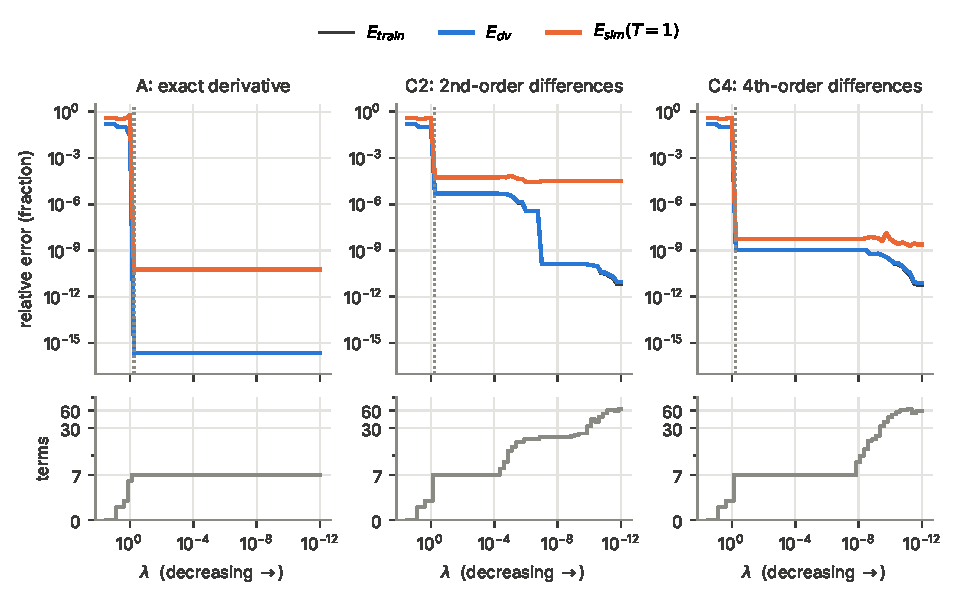
\includegraphics[width=\textwidth]{lorenz_sweep.pdf}
\caption{The three error measures against $\lambda$ ($\lambda$ decreases to the right). Lower panels: number of terms. Dotted line: $\lambda=0.56$.}
\end{figure}

\subsubsection{Comparison of rules for choosing $\lambda$}\label{sec:rules}
Four rules, each applied to $E_{dv}$ and to $E_{sim}(T{=}1)$:
\begin{enumerate}
  \item \textbf{R1:} the largest $\lambda$ whose error is within 10\% of the smallest error.
  \item \textbf{R2:} the largest $\lambda$ whose error is within a factor 10 of the smallest error.
  \item \textbf{R3:} the largest $\lambda$ whose error is below a fixed level, $10^{-3}$.
  \item \textbf{R4:} the model just after the largest drop in error (Section~\ref{sec:rule}).
\end{enumerate}
\begin{table}[H]\centering\small
\begin{tabular}{llcccc}\toprule Case & Error & R1 & R2 & R3 & R4\\\midrule
A & $E_{dv}$ & 7 (0) & 7 (0) & 7 (0) & 7 (0)\\
A & $E_{sim}(T{=}1)$ & 7 (0) & 7 (0) & 7 (0) & 7 (0)\\
C2 & $E_{dv}$ & 58 (51) & 46 (39) & 7 (0) & 7 (0)\\
C2 & $E_{sim}(T{=}1)$ & 19 (12) & 7 (0) & 7 (0) & 7 (0)\\
C4 & $E_{dv}$ & 58 (51) & 62 (55) & 7 (0) & 7 (0)\\
C4 & $E_{sim}(T{=}1)$ & 64 (57) & 7 (0) & 7 (0) & 7 (0)\\
\bottomrule\end{tabular}
\caption{Number of terms (number of wrong terms) of the model picked by each rule. The true model has 7 terms.}
\end{table}

\subsubsection{Applying R4 to Lorenz}\label{sec:lorenz-apply}
\begin{table}[H]\centering\small
\begin{tabular}{llrrcc}\toprule Case & Score & terms & wrong & $\lambda$ range of the selected model & selected $\lambda$\\\midrule
A & $E_{dv}$ & 7 & 0 & $1.0\!\times\!10^{-12}$ -- $5.6\!\times\!10^{-1}$ & $5.62\!\times\!10^{-1}$\\
A & $E_{sim}(T{=}1)$ & 7 & 0 & $1.0\!\times\!10^{-12}$ -- $5.6\!\times\!10^{-1}$ & $5.62\!\times\!10^{-1}$\\
C2 & $E_{dv}$ & 7 & 0 & $5.6\!\times\!10^{-5}$ -- $5.6\!\times\!10^{-1}$ & $5.62\!\times\!10^{-1}$\\
C2 & $E_{sim}(T{=}1)$ & 7 & 0 & $5.6\!\times\!10^{-5}$ -- $5.6\!\times\!10^{-1}$ & $5.62\!\times\!10^{-1}$\\
C4 & $E_{dv}$ & 7 & 0 & $1.8\!\times\!10^{-8}$ -- $5.6\!\times\!10^{-1}$ & $5.62\!\times\!10^{-1}$\\
C4 & $E_{sim}(T{=}1)$ & 7 & 0 & $1.8\!\times\!10^{-8}$ -- $5.6\!\times\!10^{-1}$ & $5.62\!\times\!10^{-1}$\\
\bottomrule\end{tabular}
\caption{R4 applied to every Lorenz case.}
\end{table}
The coefficients of the selected models are given in Table~\ref{tab:lorenz-coefs}.

\subsubsection{Test runs}
The selected model is scored once on the three test runs, with the same formulas as $E_{dv}$ and $E_{sim}$. The true Lorenz equations are scored on the same runs in the same way.
\begin{table}[H]\centering\small
\begin{tabular}{lllcccc}\toprule Case & Model & & $E_{dv}$ & $E_{sim}(0.5)$ & $E_{sim}(1)$ & $E_{sim}(2)$\\\midrule
A & SINDy, selected (7 terms) & & $2.2\!\times\!10^{-16}$ & $4.7\!\times\!10^{-11}$ & $3.6\!\times\!10^{-11}$ & $9.4\!\times\!10^{-11}$\\
A & true Lorenz equations & & $2.0\!\times\!10^{-17}$ & $4.7\!\times\!10^{-11}$ & $3.6\!\times\!10^{-11}$ & $9.4\!\times\!10^{-11}$\\
\addlinespace
C2 & SINDy, selected (7 terms) & & $4.9\!\times\!10^{-6}$ & $3.7\!\times\!10^{-5}$ & $4.5\!\times\!10^{-5}$ & $1.4\!\times\!10^{-4}$\\
C2 & true Lorenz equations & & $6.8\!\times\!10^{-6}$ & $4.7\!\times\!10^{-11}$ & $3.6\!\times\!10^{-11}$ & $9.4\!\times\!10^{-11}$\\
\addlinespace
C4 & SINDy, selected (7 terms) & & $1.1\!\times\!10^{-9}$ & $4.7\!\times\!10^{-9}$ & $4.8\!\times\!10^{-9}$ & $1.6\!\times\!10^{-8}$\\
C4 & true Lorenz equations & & $1.2\!\times\!10^{-9}$ & $4.7\!\times\!10^{-11}$ & $3.6\!\times\!10^{-11}$ & $9.4\!\times\!10^{-11}$\\
\bottomrule\end{tabular}
\caption{Test errors (fractions), mean over the three test runs. ODE solver tolerance: $10^{-10}$.}
\end{table}

%---------------------------------------------------------------------
\subsection{SINDy on the PDE, one frequency at a time}
SINDy is fitted separately at each of four frequencies, and the coefficients are compared with those of the Galerkin model.

\subsubsection{Training runs}
\begin{table}[H]\centering\small
\begin{tabular}{rcccc}\toprule
$\omega$ & period $P$ & $\Delta\tau=P/200$ & $\tau_{\max}=5P$ & points\\\midrule
0.1 & 62.83 & 0.3142 & 314.2 & 1001\\
1 & 6.283 & 0.03142 & 31.42 & 1001\\
10 & 0.6283 & 0.003142 & 3.142 & 1001\\
100 & 0.06283 & 0.0003142 & 0.3142 & 1001\\\bottomrule
\end{tabular}
\caption{Training runs: $\delta = A\sin(\omega\tau)$, $f=1$.}
\end{table}
\begin{itemize}
  \item Library $\{C_s,\ C_\avg,\ \delta\}$, the terms of the Galerkin model. SINDy fits only $dC_s/d\tau$; $C_\avg$ follows the mass balance, Equation~\eqref{eq:massbal}.
  \item $dC_s/d\tau$ by 2nd-order differences at all 1001 points: central differences inside, one-sided 2nd-order differences at the first and last point.
  \item The PDE data for this section come from a Python solver: Chebyshev collocation in $r$ with an implicit time integrator, tolerance $10^{-10}$. Doubling the number of radial points changes $C_s$ by less than $10^{-9}$.
\end{itemize}

\subsubsection{Validation and test data}
Four validation runs at the same $\omega$, each 10 periods long with $\Delta\tau=P/200$:
\begin{enumerate}
  \item \textbf{cos}: $\delta = A\cos(\omega\tau)$, from a uniform particle.
  \item \textbf{sin late}: periods 6 to 15 of the training sine (the PDE is continued from its state at $\tau=5P$, and the model starts from the PDE's $C_s$ and $C_\avg$ there).
  \item \textbf{sin ph}: $\delta = A\sin(\omega\tau+\pi/4)$.
  \item \textbf{cos ph}: $\delta = A\cos(\omega\tau+\pi/4)$.
\end{enumerate}
``Stacked'' is the mean of the four errors.

\textbf{Test:} the random multisine $\delta = s\sum_{k=1}^{3}a_k\sin(\omega_k\tau+\phi_k)$ with $\omega_k=\omega/2,\ \omega,\ 2\omega$, $a_k$ and $\phi_k$ as in Table~\ref{tab:random}, scaled so that $\max|\delta|=A$, 10 periods of $\omega$.
\begin{table}[H]\centering\small
\begin{tabular}{rccc}\toprule
$\omega$ & $\omega_k$ & $a_k$ & $\phi_k$\\\midrule
0.1 & 0.05, 0.1, 0.2 & 0.82, 0.74, 0.75 & 4.62, 3.09, 0.48\\
1 & 0.5, 1, 2 & 0.54, 0.91, 0.82 & 1.24, 3.70, 5.63\\
10 & 5, 10, 20 & 0.91, 0.53, 0.69 & 4.99, 2.70, 4.75\\
100 & 50, 100, 200 & 0.62, 0.97, 0.53 & 1.31, 0.81, 2.65\\\bottomrule
\end{tabular}
\caption{Parameters of the random (test) inputs.}
\label{tab:random}
\end{table}

\subsubsection{Error measures}\label{sec:pde-err}
Equation~\eqref{eq:rel} with a single variable, in \%.
\begin{itemize}
  \item $E_{sim}$: the SINDy equation for $C_s$ is solved together with $dC_\avg/d\tau=-3\delta$, from the PDE's $C_s$ and $C_\avg$ at the start of the run, and compared with the PDE's $C_s$ over the whole run:
  \[
    E_{sim}\,(\%) = 100\times\frac{\RMS\big(C_{s,\rm SINDy}-C_{s,\rm PDE}\big)}{\max C_{s,\rm PDE}-\min C_{s,\rm PDE}}\quad\text{(whole run)}.
  \]
  \item $E_{dv}$: the SINDy right-hand side, evaluated at the PDE's $C_s$, $C_\avg$ and $\delta$, against $dC_s/d\tau$ of the PDE data (2nd-order differences, as in training), whole run:
  \[
    E_{dv}\,(\%) = 100\times\frac{\RMS\big(\xi_1C_s+\xi_2C_\avg+\xi_3\delta - dC_s/d\tau\big)}{\max dC_s/d\tau-\min dC_s/d\tau}.
  \]
  \item $E_{train}$: the same as $E_{dv}$ on the training run.
\end{itemize}
$\lambda$ is chosen with the stacked $E_{sim}$.

\subsubsection{Models found}
\begin{table}[H]\centering\scriptsize\setlength{\tabcolsep}{3.5pt}
\resizebox{\textwidth}{!}{\begin{tabular}{rlrrrc|rrrr|r|rr}\toprule
 & & \multicolumn{3}{c}{coefficients} & & \multicolumn{5}{c|}{$E_{sim}$ (\%) on validation runs} & \multicolumn{2}{c}{derivative error (\%)}\\
$\omega$ & $\lambda$ range & $C_s$ & $C_{avg}$ & $\delta$ & stable & cos & sin late & sin ph & cos ph & stacked & $E_{dv}$, stacked & $E_{train}$\\\midrule
0.1 & $1.8\!\times\!10^{1}$ -- $1.0\!\times\!10^{3}$ & +0.000 & +0.000 & +0.000 & yes & 35 & 61 & 50 & 50 & 49 & 34.2 & 35.3\\
0.1 & $1.0\!\times\!10^{1}$ & +14.998 & -14.999 & +0.000 & no & $\infty$ & $\infty$ & $\infty$ & $\infty$ & $\infty$ & 0.961 & 0.144\\
\rowcolor{sel}0.1 & $1.0\!\times\!10^{-6}$ -- $5.6\!\times\!10^{0}$ & -34.638 & +34.638 & -9.927 & yes & $2.3\!\times\!10^{-5}$ & $1.7\!\times\!10^{-5}$ & $1.9\!\times\!10^{-5}$ & $2.7\!\times\!10^{-5}$ & $2.1\!\times\!10^{-5}$ & 1.26 & $9.06\!\times\!10^{-3}$\\
\midrule
1 & $1.8\!\times\!10^{1}$ -- $1.0\!\times\!10^{3}$ & +0.000 & +0.000 & +0.000 & yes & 35 & 61 & 50 & 50 & 49 & 24.4 & 35.3\\
\rowcolor{sel}1 & $1.0\!\times\!10^{-6}$ -- $1.0\!\times\!10^{1}$ & -35.039 & +35.039 & -10.004 & yes & $5.4\!\times\!10^{-3}$ & $1.8\!\times\!10^{-4}$ & $3.8\!\times\!10^{-3}$ & $3.9\!\times\!10^{-3}$ & $3.3\!\times\!10^{-3}$ & 0.136 & 0.0436\\
\midrule
10 & $1.8\!\times\!10^{1}$ -- $1.0\!\times\!10^{3}$ & +0.000 & +0.000 & +0.000 & yes & 35 & 57 & 44 & 45 & 45 & 17.4 & 35.2\\
\rowcolor{sel}10 & $1.0\!\times\!10^{-6}$ -- $1.0\!\times\!10^{1}$ & -38.077 & +38.077 & -10.313 & yes & 0.25 & 0.042 & 0.19 & 0.19 & 0.17 & 0.999 & 0.641\\
\midrule
100 & $3.2\!\times\!10^{1}$ -- $1.0\!\times\!10^{3}$ & +0.000 & +0.000 & +0.000 & yes & 35 & 52 & 35 & 35 & 39 & 16.8 & 34.5\\
100 & $1.8\!\times\!10^{1}$ & +28.745 & -28.738 & +0.000 & no & $\infty$ & $\infty$ & $\infty$ & $\infty$ & $\infty$ & 16.4 & 33.5\\
\rowcolor{sel}100 & $1.0\!\times\!10^{-6}$ -- $1.0\!\times\!10^{1}$ & -133.216 & +133.207 & -17.630 & yes & 1.7 & 1.4 & 1.5 & 2.1 & 1.7 & 1.86 & 2.82\\
\bottomrule\end{tabular}}
\caption{Models found in the $\lambda$ sweep ($10^{-6}$ to $10^3$) and their errors in \%. Each validation column is that model's $E_{sim}$ on that run. $\infty$: the solution grows without bound. The empty model keeps $C_s$ at its starting value. Shaded: the model selected by R4.}
\end{table}

\subsubsection{Choosing $\lambda$}
\begin{table}[H]\centering\scriptsize
\resizebox{\textwidth}{!}{\begin{tabular}{r|ccccc|cc|cc}\toprule
 & \multicolumn{5}{c|}{$E_{sim}$ on} & \multicolumn{2}{c|}{$E_{dv}$, stacked} & & \\
$\omega$ & cos & sin late & sin ph & cos ph & \textbf{stacked} & step 4 skipped & step 4 used & $\lambda$ range & selected $\lambda$\\\midrule
0.1 & 3 & 3 & 3 & 3 & 3 & 2, \textbf{unstable} & 3 & $1.0\!\times\!10^{-6}$ -- $5.6\!\times\!10^{0}$ & $5.6\!\times\!10^{0}$\\
1 & 3 & 3 & 3 & 3 & 3 & 3 & 3 & $1.0\!\times\!10^{-6}$ -- $1.0\!\times\!10^{1}$ & $1.0\!\times\!10^{1}$\\
10 & 3 & 3 & 3 & 3 & 3 & 3 & 3 & $1.0\!\times\!10^{-6}$ -- $1.0\!\times\!10^{1}$ & $1.0\!\times\!10^{1}$\\
100 & 3 & 3 & 3 & 3 & 3 & 3 & 3 & $1.0\!\times\!10^{-6}$ -- $1.0\!\times\!10^{1}$ & $1.0\!\times\!10^{1}$\\
\bottomrule\end{tabular}}
\caption{Number of terms of the model selected by R4 for each choice of validation error, with and without step 4 (removal of unstable models). The selection used is $E_{sim}$, stacked.}
\end{table}

\subsubsection{Test on the random input}
The selected model at each $\omega$ is scored once on the random multisine; the Galerkin model is scored on the same runs.
\begin{table}[H]\centering\small
\begin{tabular}{r|cc|cc|c}\toprule
 & \multicolumn{2}{c|}{$E_{sim}$ (\%)} & \multicolumn{2}{c|}{$E_{dv}$ (\%)} & \\
$\omega$ & Galerkin & SINDy & Galerkin & SINDy & $E_{sim}$: Galerkin / SINDy\\\midrule
0.1 & $2.02\!\times\!10^{-6}$ & $1.81\!\times\!10^{-5}$ & 0.583 & 0.576 & 0.11\\
1 & $2.18\!\times\!10^{-3}$ & $1.79\!\times\!10^{-3}$ & 0.143 & 0.13 & 1.2\\
10 & 0.756 & 0.563 & 1.61 & 1.46 & 1.3\\
100 & 11.5 & 3.93 & 4.03 & 2.38 & 2.9\\
\bottomrule\end{tabular}
\caption{Test errors on the random multisine (10 periods, whole run), in \%.}
\end{table}
\begin{figure}[H]\centering
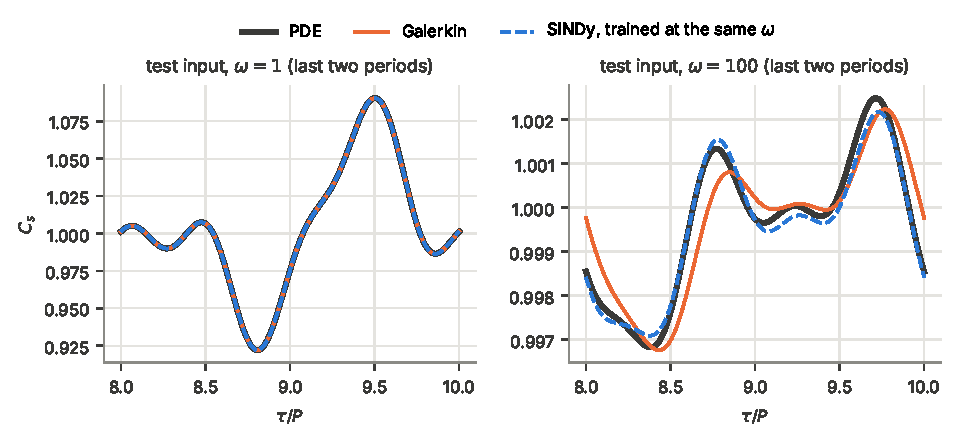
\includegraphics[width=\textwidth]{pde_test.pdf}
\caption{$C_s$ on the test input over its last two periods, at $\omega=1$ and $\omega=100$.}
\end{figure}

\subsubsection{Selected equations and the Galerkin model}
\begin{table}[H]\centering\small
\begin{tabular}{llrrr}\toprule & derivative & $C_s$ & $C_{avg}$ & $\delta$\\\midrule
Galerkin & -- & $-35$ & $+35$ & $-10$\\\midrule
$\omega=0.1$ & 2nd order & -34.638 & +34.638 & -9.927\\
 & 4th order & -34.665 & +34.665 & -9.933\\
 & 2nd order, end points dropped & -34.996 & +34.996 & -9.999\\
\addlinespace
$\omega=1$ & 2nd order & -35.039 & +35.039 & -10.004\\
 & 4th order & -35.048 & +35.048 & -10.006\\
 & 2nd order, end points dropped & -35.040 & +35.040 & -10.004\\
\addlinespace
$\omega=10$ & 2nd order & -38.077 & +38.077 & -10.313\\
 & 4th order & -38.084 & +38.084 & -10.315\\
 & 2nd order, end points dropped & -38.078 & +38.078 & -10.313\\
\addlinespace
$\omega=100$ & 2nd order & -133.216 & +133.207 & -17.630\\
 & 4th order & -133.239 & +133.229 & -17.633\\
 & 2nd order, end points dropped & -133.225 & +133.215 & -17.630\\
\bottomrule\end{tabular}
\caption{Coefficients of the selected model at each training frequency. ``End points dropped'': the same 2nd-order fit without the first and last point.}
\label{tab:pde-coefs}
\end{table}

\subsubsection{Cross-test: trained at one frequency, tested at another}
Every selected model is tested on the cosine run at each $\omega$, over the last period, with two error measures:
\begin{itemize}
  \item $C_s$: Rel (\%) of $C_s$, Equation~\eqref{eq:rel}, last period.
  \item gap: the same RMS error divided by the band of the gap $C_s-C_\avg$ instead of the band of $C_s$.
\end{itemize}
\begin{table}[H]\centering\small\setlength{\tabcolsep}{4pt}
\begin{tabular}{l|cc|cc|cc|cc}\toprule
 & \multicolumn{2}{c|}{test $\omega=0.1$} & \multicolumn{2}{c|}{test $\omega=1$} & \multicolumn{2}{c|}{test $\omega=10$} & \multicolumn{2}{c}{test $\omega=100$}\\
Model & $C_s$ & gap & $C_s$ & gap & $C_s$ & gap & $C_s$ & gap\\\midrule
Galerkin & $1.52\!\times\!10^{-6}$ & $1.61\!\times\!10^{-4}$ & $1.07\!\times\!10^{-3}$ & 0.0161 & 0.704 & 1.48 & 16.3 & 20.1\\
SINDy, trained at $\omega = 0.1$ & $2.18\!\times\!10^{-5}$ & $3.17\!\times\!10^{-3}$ & $1.15\!\times\!10^{-3}$ & 0.0174 & 0.715 & 1.51 & 16.4 & 20.3\\
SINDy, trained at $\omega = 1$ & $1.23\!\times\!10^{-4}$ & 0.0184 & $1.85\!\times\!10^{-4}$ & $2.72\!\times\!10^{-3}$ & 0.695 & 1.46 & 16.3 & 20.1\\
SINDy, trained at $\omega = 10$ & $9.40\!\times\!10^{-3}$ & 1.41 & 0.0925 & 1.39 & 0.0423 & 0.089 & 15.6 & 19.3\\
SINDy, trained at $\omega = 100$ & 0.107 & 16 & 1.06 & 16 & 7.29 & 15.4 & 1.43 & 1.77\\
\bottomrule\end{tabular}
\caption{Cross-test, Rel (\%), cosine flux, last period.}
\end{table}

%=====================================================================
\section{Summary}
\begin{itemize}
  \item Changing the flux shape changes the surface concentration response. The average concentration is set by the total charge applied, so matched pairs with the same total charge end at the same $C_\avg$ but different $C_s$.
  \item Increasing the frequency of an oscillating flux reduces the visible oscillation in $C_s$ and confines the response to a thinner layer near the surface, with the material model unchanged.
  \item Increasing the constant diffusivity makes the radial profile more uniform. The maximum gap $C_\avg-C_s$ falls from 0.0710 at $f=0.01$ to 0.000051 at $f=100$.
  \item The average concentration follows the applied flux and is essentially independent of the diffusivity, as Equation~\eqref{eq:massbal} requires.
  \item \texttt{trueRandom} gives different reproducible excitation signals for different seeds, with surface responses that are similar in character but different in detail.
  \item The Galerkin method with the two shapes 1 and $r^2-3/5$ turns the PDE into two ODEs: $dC_\avg/d\tau=-3\delta$ and $dC_s/d\tau=-35f(C_s-C_\avg)-10\,\delta$.
  \item SINDy with the library $\{C_s,C_\avg,\delta\}$ was fitted on the Lorenz system and on PDE data at $\omega=0.1$, 1, 10 and 100, with $\lambda$ chosen by rule R4; the results are in Tables~\ref{tab:lorenz-coefs} and~\ref{tab:pde-coefs}.
\end{itemize}

\appendix\sloppy
\section{Code for Experiment 6}
\begin{itemize}
  \item \textbf{Python}: \texttt{pde.py} (PDE solver and Galerkin model), \texttt{common.py} (error formula, STLSQ, rules R1--R4), \texttt{lorenz.py}, \texttt{pde\_sindy.py}, \texttt{figures.py}, \texttt{tables.py}.
  \item \textbf{MATLAB}: \texttt{relErr.m}, \texttt{stlsq.m}, \texttt{lambdaGrid.m}, \texttt{sweepLambda.m}, \texttt{selectLambdaR4.m}, \texttt{solvePDE.m} (uses \texttt{pdepe} when available, otherwise a Chebyshev method of lines), \texttt{galerkinModel.m}, \texttt{run\_lorenz.m}, \texttt{run\_pde\_omega.m}, \texttt{run\_pde\_all.m}, \texttt{test\_quick.m}.
\end{itemize}

\end{document}
